\documentclass[a4paper,11pt]{article}
\usepackage[a4paper, margin=8em]{geometry}

% usa i pacchetti per la scrittura in italiano
\usepackage[french,italian]{babel}
\usepackage[T1]{fontenc}
\usepackage[utf8]{inputenc}
\frenchspacing 

% usa i pacchetti per la formattazione matematica
\usepackage{amsmath, amssymb, amsthm, amsfonts}

% usa altri pacchetti
\usepackage{gensymb}
\usepackage{hyperref}
\usepackage{standalone}

\usepackage{colortbl}

\usepackage{xstring}
\usepackage{karnaugh-map}

% imposta il titolo
\title{Appunti Reti Informatiche}
\author{Luca Seggiani}
\date{2025}

% imposta lo stile
% usa helvetica
\usepackage[scaled]{helvet}
% usa palatino
\usepackage{palatino}
% usa un font monospazio guardabile
\usepackage{lmodern}

\renewcommand{\rmdefault}{ppl}
\renewcommand{\sfdefault}{phv}
\renewcommand{\ttdefault}{lmtt}

% circuiti
\usepackage{circuitikz}
\usetikzlibrary{babel}

% testo cerchiato
\newcommand*\circled[1]{\tikz[baseline=(char.base)]{
            \node[shape=circle,draw,inner sep=2pt] (char) {#1};}}

% disponi il titolo
\makeatletter
\renewcommand{\maketitle} {
	\begin{center} 
		\begin{minipage}[t]{.8\textwidth}
			\textsf{\huge\bfseries \@title} 
		\end{minipage}%
		\begin{minipage}[t]{.2\textwidth}
			\raggedleft \vspace{-1.65em}
			\textsf{\small \@author} \vfill
			\textsf{\small \@date}
		\end{minipage}
		\par
	\end{center}

	\thispagestyle{empty}
	\pagestyle{fancy}
}
\makeatother

% disponi teoremi
\usepackage{tcolorbox}
\newtcolorbox[auto counter, number within=section]{theorem}[2][]{%
	colback=blue!10, 
	colframe=blue!40!black, 
	sharp corners=northwest,
	fonttitle=\sffamily\bfseries, 
	title=Teorema~\thetcbcounter: #2, 
	#1
}

% disponi definizioni
\newtcolorbox[auto counter, number within=section]{definition}[2][]{%
	colback=red!10,
	colframe=red!40!black,
	sharp corners=northwest,
	fonttitle=\sffamily\bfseries,
	title=Definizione~\thetcbcounter: #2,
	#1
}

% disponi codice
\usepackage{listings}
\usepackage[table]{xcolor}

\definecolor{codegreen}{rgb}{0,0.6,0}
\definecolor{codegray}{rgb}{0.5,0.5,0.5}
\definecolor{codepurple}{rgb}{0.58,0,0.82}
\definecolor{backcolour}{rgb}{0.95,0.95,0.92}

\lstdefinestyle{codestyle}{
		backgroundcolor=\color{black!5}, 
		commentstyle=\color{codegreen},
		keywordstyle=\bfseries\color{magenta},
		numberstyle=\sffamily\tiny\color{black!60},
		stringstyle=\color{green!50!black},
		basicstyle=\ttfamily\footnotesize,
		breakatwhitespace=false,         
		breaklines=true,                 
		captionpos=b,                    
		keepspaces=true,                 
		numbers=left,                    
		numbersep=5pt,                  
		showspaces=false,                
		showstringspaces=false,
		showtabs=false,                  
		tabsize=2
}

\lstdefinestyle{shellstyle}{
		backgroundcolor=\color{black!5}, 
		basicstyle=\ttfamily\footnotesize\color{black}, 
		commentstyle=\color{black}, 
		keywordstyle=\color{black},
		numberstyle=\color{black!5},
		stringstyle=\color{black}, 
		showspaces=false,
		showstringspaces=false, 
		showtabs=false, 
		tabsize=2, 
		numbers=none, 
		breaklines=true
}


\lstdefinelanguage{assembler}{ 
  keywords={AAA, AAD, AAM, AAS, ADC, ADCB, ADCW, ADCL, ADD, ADDB, ADDW, ADDL, AND, ANDB, ANDW, ANDL,
        ARPL, BOUND, BSF, BSFL, BSFW, BSR, BSRL, BSRW, BSWAP, BT, BTC, BTCB, BTCW, BTCL, BTR, 
        BTRB, BTRW, BTRL, BTS, BTSB, BTSW, BTSL, CALL, CBW, CDQ, CLC, CLD, CLI, CLTS, CMC, CMP,
        CMPB, CMPW, CMPL, CMPS, CMPSB, CMPSD, CMPSW, CMPXCHG, CMPXCHGB, CMPXCHGW, CMPXCHGL,
        CMPXCHG8B, CPUID, CWDE, DAA, DAS, DEC, DECB, DECW, DECL, DIV, DIVB, DIVW, DIVL, ENTER,
        HLT, IDIV, IDIVB, IDIVW, IDIVL, IMUL, IMULB, IMULW, IMULL, IN, INB, INW, INL, INC, INCB,
        INCW, INCL, INS, INSB, INSD, INSW, INT, INT3, INTO, INVD, INVLPG, IRET, IRETD, JA, JAE,
        JB, JBE, JC, JCXZ, JE, JECXZ, JG, JGE, JL, JLE, JMP, JNA, JNAE, JNB, JNBE, JNC, JNE, JNG,
        JNGE, JNL, JNLE, JNO, JNP, JNS, JNZ, JO, JP, JPE, JPO, JS, JZ, LAHF, LAR, LCALL, LDS,
        LEA, LEAVE, LES, LFS, LGDT, LGS, LIDT, LMSW, LOCK, LODSB, LODSD, LODSW, LOOP, LOOPE,
        LOOPNE, LSL, LSS, LTR, MOV, MOVB, MOVW, MOVL, MOVSB, MOVSD, MOVSW, MOVSX, MOVSXB,
        MOVSXW, MOVSXL, MOVZX, MOVZXB, MOVZXW, MOVZXL, MUL, MULB, MULW, MULL, NEG, NEGB, NEGW,
        NEGL, NOP, NOT, NOTB, NOTW, NOTL, OR, ORB, ORW, ORL, OUT, OUTB, OUTW, OUTL, OUTSB, OUTSD,
        OUTSW, POP, POPL, POPW, POPB, POPA, POPAD, POPF, POPFD, PUSH, PUSHL, PUSHW, PUSHB, PUSHA, 
				PUSHAD, PUSHF, PUSHFD, RCL, RCLB, RCLW, MOVSL, MOVSB, MOVSW, STOSL, STOSB, STOSW, LODSB, LODSW,
				LODSL, INSB, INSW, INSL, OUTSB, OUTSL, OUTSW
        RCLL, RCR, RCRB, RCRW, RCRL, RDMSR, RDPMC, RDTSC, REP, REPE, REPNE, RET, ROL, ROLB, ROLW,
        ROLL, ROR, RORB, RORW, RORL, SAHF, SAL, SALB, SALW, SALL, SAR, SARB, SARW, SARL, SBB,
        SBBB, SBBW, SBBL, SCASB, SCASD, SCASW, SETA, SETAE, SETB, SETBE, SETC, SETE, SETG, SETGE,
        SETL, SETLE, SETNA, SETNAE, SETNB, SETNBE, SETNC, SETNE, SETNG, SETNGE, SETNL, SETNLE,
        SETNO, SETNP, SETNS, SETNZ, SETO, SETP, SETPE, SETPO, SETS, SETZ, SGDT, SHL, SHLB, SHLW,
        SHLL, SHLD, SHR, SHRB, SHRW, SHRL, SHRD, SIDT, SLDT, SMSW, STC, STD, STI, STOSB, STOSD,
        STOSW, STR, SUB, SUBB, SUBW, SUBL, TEST, TESTB, TESTW, TESTL, VERR, VERW, WAIT, WBINVD,
        XADD, XADDB, XADDW, XADDL, XCHG, XCHGB, XCHGW, XCHGL, XLAT, XLATB, XOR, XORB, XORW, XORL},
  keywordstyle=\color{blue}\bfseries,
  ndkeywordstyle=\color{darkgray}\bfseries,
  identifierstyle=\color{black},
  sensitive=false,
  comment=[l]{\#},
  morecomment=[s]{/*}{*/},
  commentstyle=\color{purple}\ttfamily,
  stringstyle=\color{red}\ttfamily,
  morestring=[b]',
  morestring=[b]"
}

\lstset{language=assembler, style=codestyle}

% disponi sezioni
\usepackage{titlesec}

\titleformat{\section}
	{\sffamily\Large\bfseries} 
	{\thesection}{1em}{} 
\titleformat{\subsection}
	{\sffamily\large\bfseries}   
	{\thesubsection}{1em}{} 
\titleformat{\subsubsection}
	{\sffamily\normalsize\bfseries} 
	{\thesubsubsection}{1em}{}

% tikz
\usepackage{tikz}

% float
\usepackage{float}

% grafici
\usepackage{pgfplots}
\pgfplotsset{width=10cm,compat=1.9}

% disponi alberi
\usepackage{forest}

\forestset{
	rectstyle/.style={
		for tree={rectangle,draw,font=\large\sffamily}
	},
	roundstyle/.style={
		for tree={circle,draw,font=\large}
	}
}

% disponi algoritmi
\usepackage{algorithm}
\usepackage{algorithmic}
\makeatletter
\renewcommand{\ALG@name}{Algoritmo}
\makeatother

% disponi numeri di pagina
\usepackage{fancyhdr}
\fancyhf{} 
\fancyfoot[L]{\sffamily{\thepage}}

\makeatletter
\fancyhead[L]{\raisebox{1ex}[0pt][0pt]{\sffamily{\@title \ \@date}}} 
\fancyhead[R]{\raisebox{1ex}[0pt][0pt]{\sffamily{\@author}}}
\makeatother

\begin{document}
% sezione (data)
\section{Lezione del 22-10-25}

% stili pagina
\thispagestyle{empty}
\pagestyle{fancy}

% testo
\subsection{LAN}
Le reti \textbf{LAN} (\textit{Local Area Network}) sono reti ad accesso \textit{locale}, quindi di estensione più o meno limitata ma comunque nell'ordine di abitazioni, edifici o al limite insiemi di edifici. La velocità in bitrate si aggira fra le centinaia di Mbps e le decine di Gbps.

Sono reti che sfruttano mezzi di tipo \textit{broadcast}, e quindi richiedono sia un protcollo MAC per l'\textit{accesso al mezzo}, che un meccanismo di \textbf{indirizzamento MAC}.

Il mezzo trasmissivo condiviso può assumere diverse topologie, cioè vi possono essere diverse \textit{topologie di rete}.
Ad esempio, possiamo nominare: 

\newpage

\begin{itemize}
	\item 
		Topologia a \textbf{stella}, dove un nodo centrale detto \textit{hub} connette più nodi periferici:
		\begin{center}
			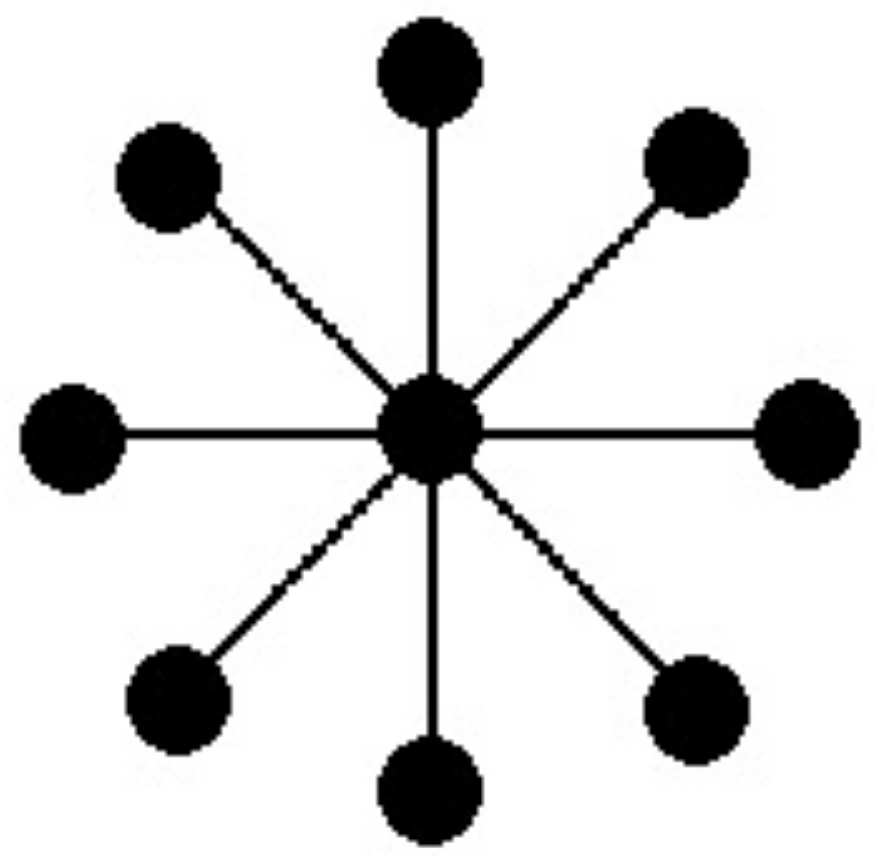
\includegraphics[scale=0.11]{../figures/star.png}
		\end{center}
		Viene detta anche \textit{bus in the box}, in quanto l'hub rappresenta effettivamente una sorta di "bus" avvolto su sé stesso. Dal punto di vista elettronico l'hub non sarà altro che un amplificatore operazionale che amplifica il segnale e lo inoltra agli altri nodi;
	\item Topologia a \textbf{ring}, dove ogni nodo è collegato a 2 nodi adiacenti in una struttura circolare:
		\begin{center}
			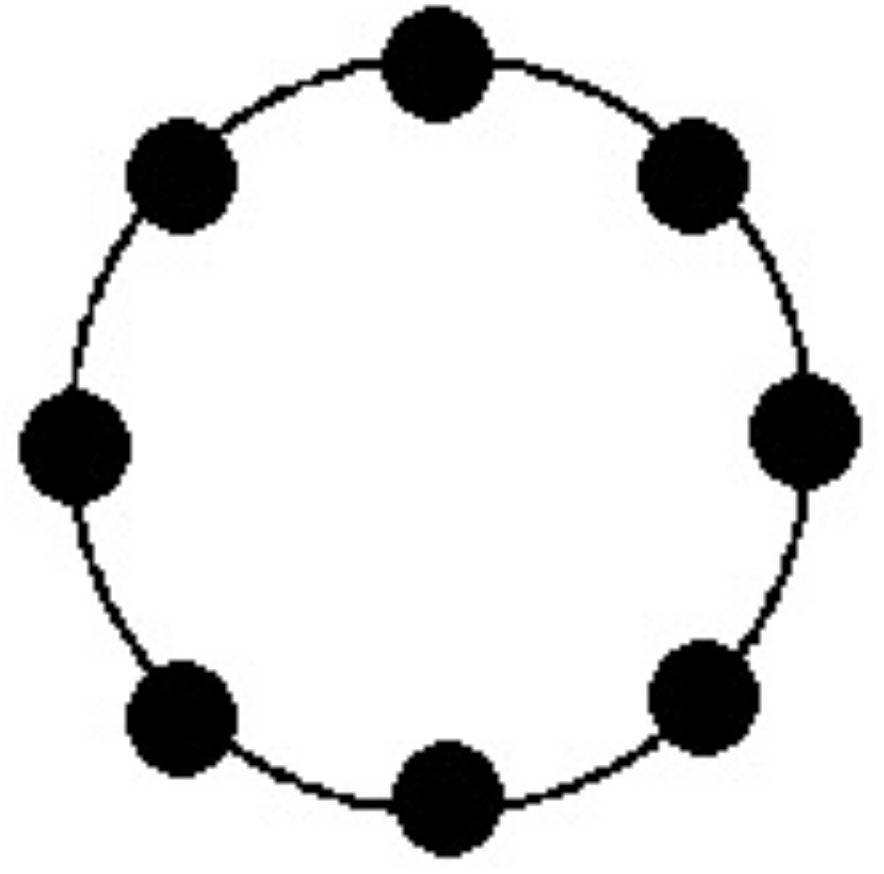
\includegraphics[scale=0.11]{../figures/ring.png}
		\end{center}
	\item Topologia a \textbf{bus}, dove tutti i nodi condividono un'unica linea di comunicazione condivisa:
		\begin{center}
			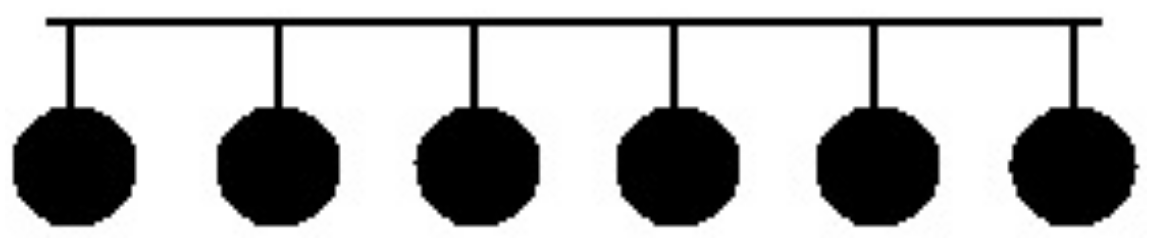
\includegraphics[scale=0.11]{../figures/bus.png}
		\end{center}
		Gli hub, dal punto di vista elettronico, dovranno essere \textit{"smorzati"} con una resistenza che ne ancori il valore quando questi non portano segnale. Questa viene detta \textit{terminatore}.
\end{itemize}

\subsubsection{Indirizzamento MAC}
Gli indirizzi \textbf{MAC} (detti anche indirizzi \textit{fisici}, \textit{LAN} o \textit{Ethernet}) vengono usati per inviare frame fra interfacce localmente e fisicamente connesse fra di loro (cioé stanti su rete LAN).
L'indirizzo MAC è su 48 bit, solitamente incluso nel firmware della NIC, a volte configurabile da software.
I primi 24 bit dei codici MAC sono solitamente assegnati (dalla IEEE) all'azienda produttrice della NIC.
Le aziende acquistano infatti porzioni dello spazio di indirizzamento MAC, per garantire l'univocità. 
I bit sucessivi sono quindi univoci per i singoli prodotti (magari hanno bit superiori dedicati a codificare categorie di prodotti, ecc...).

Ai MAC associamo chiaramente gli indirizzi \textbf{IP} su 32 bit che abbiamo già visto più volte. Ricordiamo che questi vengono usati a livello 3, cioè livello network, per effettuare il cosiddetto \textit{packet forwarding}. Noi adesso stiamo discutendo il livello 1, cioè livello link.

Una buona analogia per il rapporto fra MAC e IP è questa:
\begin{itemize}
	\item L'indirizzo \textbf{MAC} è il \textit{codice fiscale};
	\item L'indirizzo \textbf{IP} è l'\textit{indirizzo di casa}.
\end{itemize}

Chiaramente, il MAC è unico per tutti, mentre l'IP può cambiare. Può essere che lo stesso dispositivo apparga, con lo stesso MAC, a più indirizzi IP nel tempo.

\subsection{Ethernet}
\textbf{Ethernet} è una famiglia di tecnologie, dominanti nell'ambito delle reti locali (LAN) cablate.

\subsubsection{Old fashioned Ethernet}
Ethernet è stata la prima tecnologia LAN ampiamente usata. Semplice ed economica, nelle sue prime versioni (\textit{old fashioned Ethernet}) sfruttava come mezzo un cavo coassiale usato come bus da più dispositivi.
I dispositivi si allacciavano al bus attraverso i cosiddetti \textit{tap} (spesso perforazioni dirette del cavo coassiale), e il bus veniva terminato con una resistenza da 50 Ohm.
La velocità di trasmissione era di 10 Mbps.

\subsubsection{Ethernet oggi}
Oggi Ethernet non sfrutta più bus su cavi coassiali, ma dispositivi di hub (detti \textit{switch}). La differenza precisa fra hub e switch verrà discussa in seguito.

I nodi si collegano all'hub attraverso il classico doppino telefonico (per Ethernet con connettore RJ48.

\par\smallskip

Ethernet è un protocollo di tipo:
\begin{itemize}
	\item \textbf{Senza connessione}: non c'è nessuna forma di \textit{handshaking} fra le NIC trasmettitore e ricevitore;
	\item \textbf{Inaffidabile}: le NIC ricevitore non trasmettono ACK o NAK alle NIC trasmettitore. I dati nei frame persi vengono recuperati solo se il mittente usa un protocollo di trasferimento dati affidabile (ad esempio TCP);
	\item Il protocollo \textbf{MAC} di Ethernet è \textit{CSMA/CD unslotted} con \textit{backoff binario}.
\end{itemize}

\subsubsection{Frame Ethernet}
Un \textbf{frame Ethernet} incapsula un datagramma IP (o un qualche altro pacchetto di protocollo network) in una struttura del tipo:
\begin{lstlisting}[style=codestyle]
8 byte			6 byte	6 byte	6 byte	variabile	4 byte
<preamble>	<dest>	<src>		<type>	<data>		<crc>
\end{lstlisting}
\begin{itemize}
	\item \lstinline|preamble| viene usato per avere sincronia fra ricevitore e tramsettitore: consiste in 7 byte di \lstinline|10101010| seguiti da un byte di \lstinline|10101011|.

	Può essere utile una breve discussione di come si trasmettono le sequenze di bit su Ethernet: anziché trasmettere i bit come 1 o 0 fisici, si trasmettono come transizioni da 1 a 0 e viceversa. Ciò si ottiene facilmente modulando i dati in XOR con il clock del trasmettitore.

		Questo permette al ricevitore di rilevare transizioni anziché valori statici, e permette quindi nella fase (piuttosto lunga) di trasmissione del preambolo, la sincronizzazione dei clock.
		
	\item Gli indirizzi \lstinline|dest| e \lstinline|src| (rispettivamente \textit{destinazione} e \textit{sorgente}) sono su 6 byte, e sono di tipo MAC. Quando l'adattatore Ethernet riceve un frame con indirizzo MAC che combacia col suo (oppure un indirizzo broadcast, ad esempio per un pacchetto \textit{ARP}, che vedremo fra poco), inoltra i dati incapsulati nel frame (campo \lstinline|data|) al livello network. In caso contrario ignora il frame;
	\item \lstinline|data| è il campo dati, cioè trasporta il \textit{payload} (il datagramma IP o simile). Ha dimensione variabile dai 48 ai 1500 byte. 

		\begin{itemize}
			\item La dimensione massima $L_\text{max} = 1500 \, \text{bit}$ è fissata per evitare la degradazione del segnale. Ethernet prevedeva infatti una distanza massima di 500m di cavo (200m per cavi più sottili), e l'introduzione di \textbf{repeater} (\textit{ripetitori}) per raggiungere distanze maggiori (fino a 4 in cascata, per un totale di 2.5 Km di copertura).
			\item La dimensione minima $L_\text{min} = 42 \, \text{bit}$ è legata al rilevamento di collisioni su vecchio Ethernet coassiale.

Se poniamo come $\tau$ il tempo di propagazione da host a ripetitore, o da ripetitore a ripetitore, abiamo che su una linea di distanza massima (4 ripetitori) il tempo di rilevamenteo di collisione è:
$$
t_\text{coll} = 2 \tau + \Delta R = \frac{2 l_\text{max}}{v} + \Delta R \leq \frac{L_\text{min}}{R}
$$
dove $l_\text{max} = 500 \, \text{m}$ è la distanza del link, e $v$ la velocità di propagazione sul mezzo (per il rame circa 200.000 Km al secondo). $\Delta R$ è invece un ritardo dovuto al repeater attraversato.
$L_\text{min}$ sarà quindi la lunghezza minima del frame in modo che le collisioni possano essere rilevate in tempo utile (prima della completa trasmissione del frame). Abbiamo già messo a diseguaglianza il tempo di trasmissione $L_\text{min} / R$, quindi ricaviamoci $L_\text{min}$:
$$
L_\text{min} \geq \left( \frac{2 l_\text{max}}{v} + \Delta R \right) R
$$
Il valore di 48 byte si ricava esattamente in questo modo.

		\end{itemize}

	\item \lstinline|type| indica il protocollo di livello network (solitamente IP);
	\item \lstinline|crc| è un campo di ridondanza che permette il rilevamento di errori al ricevitore. I frame corrotti vengono persi.
\end{itemize}

Chiaramente, la privacy dei frame non è assicurata: ci potremmo fidare che tutte le interfacce NIC ignorano i frame che non le spettano, ma è possibile configurarle nella cosiddetta \textbf{modalità promiscua} per costringerle a rilevare tutti i frame, qualsiasi sia il destinatario.

L'\textbf{indirizzo di broadacst} è un indirizzo particolare a cui tutti i nodi rispondono (cioè da cui tutti i nodi ricevono frame), e viene usato, appunto, per fare \textit{broadcast} di frame destinati alla totalità dei dispositivi in rete.

\subsubsection{CSMA/CD su Ethernet}
Vediamo come Ethernet implementa il protocollo CSMA/CD per permettere la condivisione del mezzo (MAC).

\begin{enumerate}
	\item Quando la NIC riceve dati dal livello network, crea un frame;
	\item Se la NIC rileva il mezzo fermo per 96 unità di tempo bit (con bitrate di 10 Mbps, 9.6 ms), e quindi trasmette;
	\item Se la NIC riesce a trasmettere l'intero frame senza collisioni, il suo lavoro è finito;
	\item Se la NIC rileva una collisione, abortisce ed invia un segnale di jam da 48 bit;
\item Dopo aver abortito, la NIC entra in \textit{backoff esponenziale} come già visto in 13.1.7: quindi sceglie un $K$ casuale fra ${0, 1, 2, ..., 2^m - 1}$ alla $m$-esima iterazione, aspetta $K \cdot 512$ tempi bit, e torna al passo 2. Dopo 17 tentativi il frame è perso.
\end{enumerate}

\subsubsection{Livelli datalink e physical in Ethernet}
Ethernet è definito da una vasta gamma di \textit{standard} (100BASE-TX, 100BASE-T2, 100BASE-FX, 100BASE-T4, 100BASE-SX, 100BASE-BX), che hanno in comune il protocollo MAC e il formato dei frame. Le velocità invece differiscono ampiamente: 2, 10, 100 Mbps, oppure 1, 10, 40 Gbps.

Questi standard definiscono informazioni utili al livello \textbf{datalink} (o semplicemente \textit{link}) e \textbf{physical}.
Abbiamo infatti già introdotto come il vecchio Ethernet sfruttava, al livello fisico, bus su cavi coassiali, mentre oggi sfrutta collegamenti punto-punto (via doppino telefonico) dai nostri dispositivi ad un unico switch Ethernet centralizzato.

\end{document}
